\section{Тэсціраванне вэб-праекта}

Тэсціраванне праграмнага забеспячэння --- працэс даследвання, выпрабавання праграмнага прадукту
(у нашым выпадку вэб-сайт), які мае сваёй мэтай праверку адпаведнасці паміж рэальнымі паводзінамі праграмы
і яе чаканымі паводзінамі пры дапамозе набору тэстаў, абраныя пэўным чынам.

\subsection{Функцыянальнае тэсціраванне}

Функцыянальнае тэсціраванне --- гэта тэсціраванне праграмнага забеспячэння ў мэтах праверкі
рэалізаванасці функцыянальных патрабаваннях, гэта значыць здольнасці праграмнага забеспячэння
ў пэўных умовах рашаць задачы, патрэбныя карыстальнікам. Функцыянальныя патрабаванні вызначаюць,
што іменна робіць праграмнае забеспячэнне, якія задачы яно рашае.

Функцыянальныя патрабаванні ўключаюць у сябе:
\begin{enumerate}
    \item функцыянальная прыдатнасць;
    \item дакладнасць;
    \item здольнасць да ўзаемадзеяння;
    \item адпаведнасць стандартам і правілам;
    \item абароненасць.
\end{enumerate}

Для напісання функцыянальных тэстаў быў абраны фрэймворк PyTest, напісаны на
мовe праграмавання Python.

На лістынгу \ref{lst: pytest code} прадстаўлены зыходны код для тэстаў.
 
\lstinputlisting[caption={Зыходны код для тэстаў},%
                            label={lst: pytest code},%
                            language=Python]{function_test.py}

З лістынга \ref{lst: pytest code} бачым, што тэсты правяраюць наступныю функцыянальсць вэб-сайта:
\begin{enumerate}
    \item наяўнасць доступу да html-старонак (правяраецца статус код у адказе);
    \item працаздольнасць пошуку кніг па аўтару (пасылаецца запыт з адпаведнымі параметрамі і
          правяраецца ці ёсць кніга аўтара на html-старонцы ў адказе);
    \item працаздольнасць пошуку кніг па назве (пасылаецца запыт з адпаведнымі параметрамі і
          правяраецца ці ёсць кніга з патрэбнай назвай на html-старонцы ў адказе);
    \item немагчымасць зарэгістраваць карыстальніка з паўторным іменем (пасылаецца POST запыт і
          правяраецца наяўнасць памылкі на html-старонцы ў адказе).
\end{enumerate}

На малюнку \ref{img: pytest output} прадстаўлены вынік запуску функцыянальных тэстаў.
\begin{figure}[h!]
    \centering
    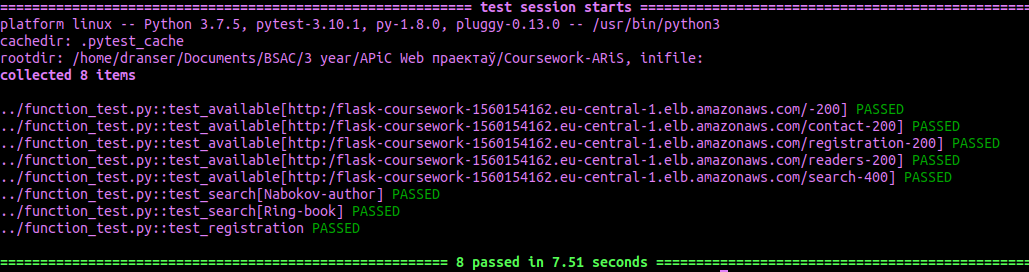
\includegraphics[width=\textwidth]{pytest_output}
    \caption{Вынік функцыянальных тэстаў}
    \label{img: pytest output} 
\end{figure}

Згодна з малюнкам \ref{img: pytest output} можам сцвярджаць, што распрацаваны вэб-сайт
выконвае вышэй апісаныя функцыя.

\subsection{Нагрузачнае тэсціраванне}

Нагрузачнае тэсціраванне --- падвід тэсціравання прадукцыйнасці, збор паказальнікаў і вызначэнне
прадукцыйнасці і часу водгуку праграмна-тэхнічнай сістэмы альбо прылады ў адказ на вонкавы запыт
з мэтай устанаўлення адпаведнасці патрабаванням, якія прад'яўляюцца да дадзенай сістэмы (прылады).
Для даследвання часу водгуку сістэмы на высокіх альбо пікавых нагрузках робіцца стрэс-тэсціраванне,
падчас якога нагрузка, што ствараецца на сістэму, перавышае нармальны сцэнар яе карыстання.

Для нагрузачнага праграмавання будзе выкарыстоўвацца праграма httperf.
httperf --- гэта праграма, якая дазваляе выконваць аўтаматычнае нагрузачнае тэсціраванне веб-сервера.
Праграма дазваляе вызначаць паводзіны статычных вэб-старонак, CGI прадукцыйнасць, SSL прадукцыйнасць.
httperf падтрымлівае HTTP/1.0 і HTTP/1.1 і дазваляе сімуляваць сесіі, каторыя падобныя да сесій карыстальнікаў.

На лістынгу \ref{lst: httperf command} прадстаўлена каманда запуску httperf.

\begin{lstlisting}[language=bash,caption={Каманда запуску праграмы httperf},label={lst: httperf command}]
httperf --server flask-coursework-1560154162.eu-central-1.elb.amazonaws.com \
        --port 80 --uri / \
        --rate 150 --num-conn 1000 \
        --num-call 1 --timeout 5 \
        --verbose
\end{lstlisting}

Апішам аргументы праграмы, якімі карысталіся:
\begin{enumerate}
    \item server --- базавае DNS імя веб-сайта;
    \item port --- порт, на які будуць адпраўляцца запыты;
    \item uri --- старонка (файл), які мы жадаем загрузіць;
    \item rate --- колькасць запытаў на секунду;
    \item num-conn --- агульная колькасць TCP падключэнняў;
    \item num-call --- колькасць запытаў на кожнае падключэнне;
    \item timeout --- час, праз які будзе лічыцца, што запыт пацярпеў няўдачу;
    \item verbose --- падрабязны вывад праграмы.
\end{enumerate}

На малюнку \ref{img: httperf output} прадстаўлены вынікі нагрузачнага тэста.
\begin{figure}[h!]
    \centering
    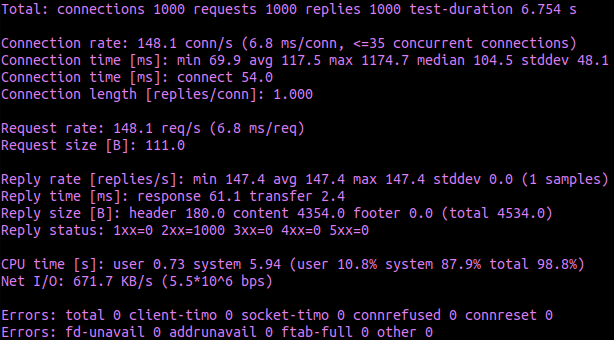
\includegraphics[width=0.7\textwidth]{httperf_output}
    \caption{Вынік нагрузачнага тэста}
    \label{img: httperf output} 
\end{figure}

З малюнка \ref{img: httperf output} можам вызначыць, што вэб-сервер электроннай
бібліятэкі можа абслугоўваць да 1000 карыстальнікаў адначасова з добрым узроўнем якасці.
Можам бачыць, што для 148 падключэнняў на секунду час падключэння у сярэднім складае 117 мс,
час атрымання html-старонкі 147,4 мс адпаведна і не было ніводнага памылкі (кожнае падключэнне
атрымала код адказу 2хх).
Неабходна заўважыць, што пры падключэнні 1000 карыстальнікаў адначасова CPU сервера загружаецца
амаль на 100\%. Гэта значыць, што пры павелічэнні колькасць карыстальнікаў электроннай бібліятэкі
неабходна ўстанаўліваць сігналы для ASG, каб у залежнасці ад загрузкі CPU альбо колькасці падключэнняў
аўтаматычна разгортвалася новая віртуальная машына ў ASG, пры вяртанні параметраў у ранейшыя значэнні ---
знішчала віртуальную машыну (гарызантальнае маштабаванне).
